\newpage

\section{Diagrama de sequência}

Visto que a realização da autenticação, ativação e confirmação de conta requer passos extras e regras a seguir, 
foi necessário criar diagramas de sequência para especificar a sequência de interações do com o sistema.

\subsection{Diagrama de sequência Login e ativação de conta}

Através deste diagrama (Figura~\ref{fig:30}) é entende-se que assim que o técnico deseja realizar o 
login, primeiramente tem de verificar as credenciais, caso estas se encontrem incorretas, este receberá 
uma mensagem de erro, caso as credenciais estejam válidas e a conta esteja ativada o técnico ficará 
autenticado. 

Caso o técnico coloque as credenciais corretas, mas a conta não esteja ativada, este irá realizar a 
ativação de conta, onde poderá enviar o código de ativação, caso esteja correto a sua conta será 
ativada, caso contrário este receberá uma mensagem de erro. Este poderá também cancelar a 
ativação de conta e pedir um novo email de ativação, onde será pedido novo código ao servidor, 
este será gerado e enviado.

\begin{figure}[htb]
    \centering
    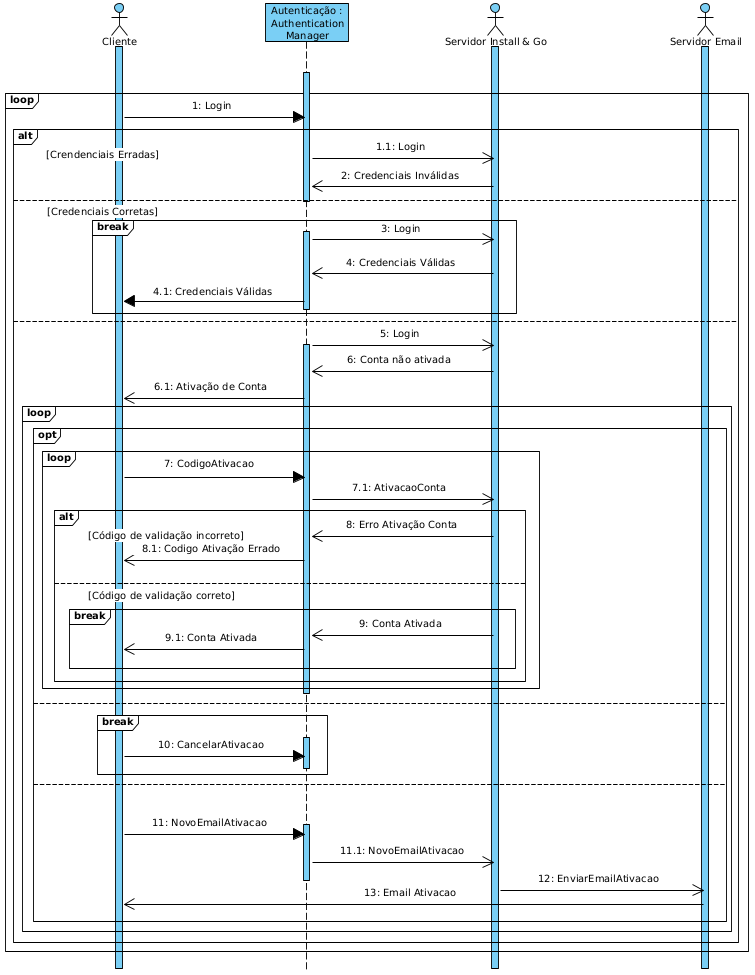
\includegraphics[width=0.67\textwidth]{images/diagramas/sequencia/diagrama_login.png}
    \caption{Diagrama de sequência de login e ativação de conta}
    \label{fig:30}
\end{figure}

\newpage

\subsection{Diagrama de sequência Registo e ativação de conta}

Através do diagrama abaixo representado (Figura~\ref{fig:31}) é possível perceber que quando uma
empresa realiza o registo este será enviado para o servidor, o qual registará a empresa com uma 
conta não ativada, esta conta será então validada pela Motorline sendo de seguida
gerado um código de ativação e enviado por email para o 
email de registo, após isto a empresa será encaminhado para a validação de conta, esta validação 
ocorre seguindo o mesmo processo mencionado no anteriormente.


\begin{figure}[htb]
    \centering
    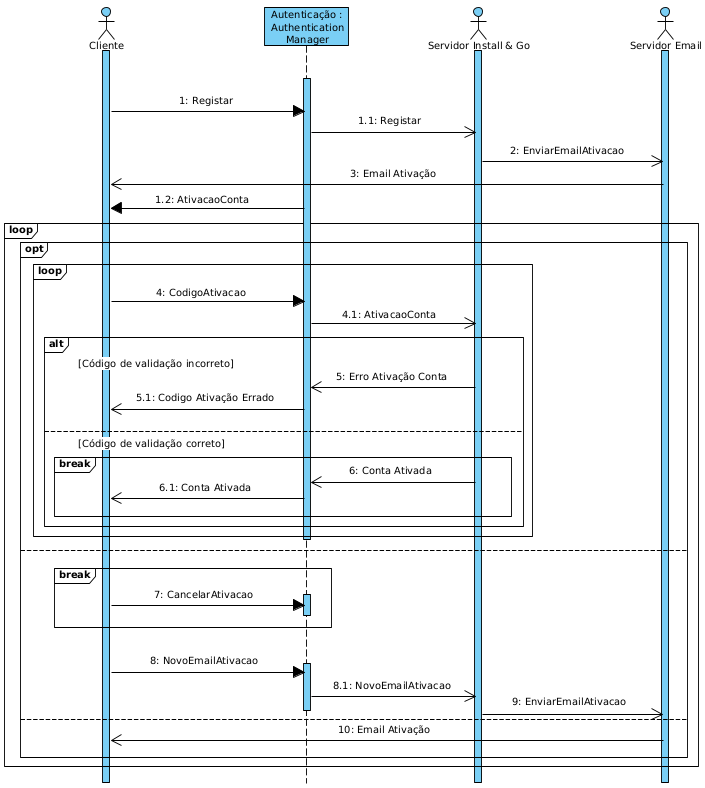
\includegraphics[width=0.8\textwidth]{images/diagramas/sequencia/diagrama_registo.png}
    \caption{Diagrama de sequência de registo e validação de conta}
    \label{fig:31}
\end{figure}

\newpage

\subsection{Diagrama de sequência registo de técnicos}

Através do diagrama abaixo representado (Figura~\ref{fig:32}) é possível perceber que quando uma
empresa deseja registar um técnico, esta introduzirá os seus dados, sendo a sua conta criada. Após isto, 
um código de ativação é gerado e enviado para o técnico ativar a sua conta.

\begin{figure}[htb]
    \centering
    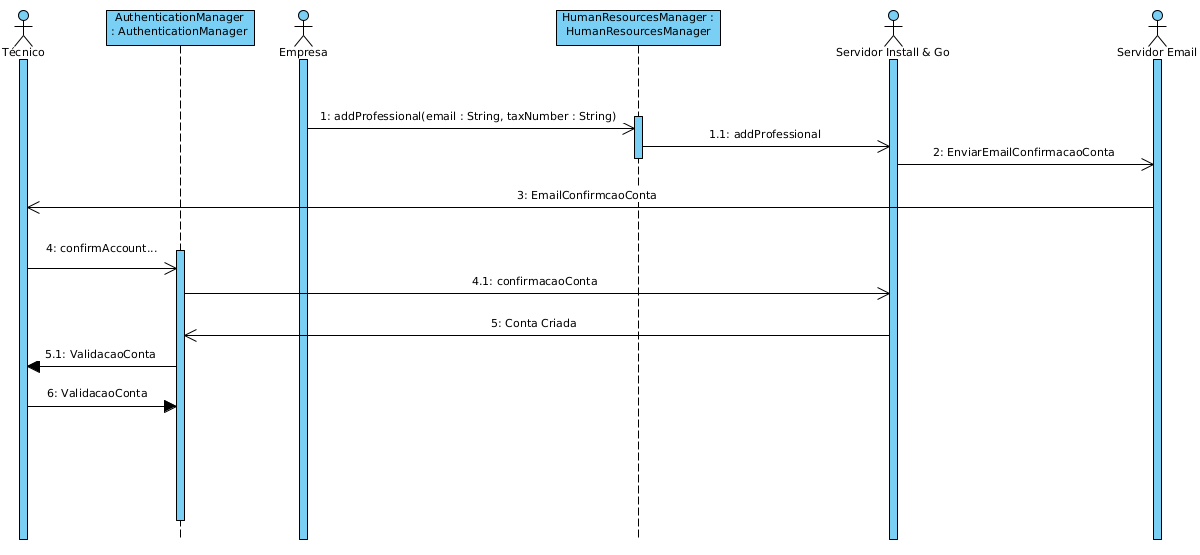
\includegraphics[width=0.8\textwidth]{images/diagramas/sequencia/registo_tecnico.png}
    \caption{Diagrama de sequência de registo de técnicos}
    \label{fig:32}
\end{figure}